In Hops in order to communicate with the MySQL Cluster NDB we make use
of ClusterJ \cite{clusterj}, a high level API to perform
operations on NDB. In a sense it is similar to other ORM frameworks
such as Hibernate \cite{hibernate} and EclipseLink \cite{eclipselink}
which provide an object-relational mapping but more lightweight and is
designed to provide high performance methods for storing and accessing
data on a MySQL Cluster from a Java application. Every operation on
Hops and Hops-YARN, except for the events received from the NDB Event
API, goes through ClusterJ which in turn uses the C++ NDB API. The
mapping between a table-oriented view and a Java object is done
through specially decorated interfaces. The interface provides signatures
for the getters and setters methods.

For example Listing \ref{lst:clusterj_intf} shows the interface for
accessing database entries for the Garbage Collector service regarding
old RPCs. The interface is annotated with the table name and contains
signatures for accessing each column of the table. The methods are
also decorated with the primary key annotation and the column
name. For every table in the database there exists such an interface
and all the operations from Hops-YARN are done on the \emph{Data
  Transfer Objects} (DTO) defined
by the annotated interfaces. DTOs are
created from a \emph{session} object which represent a connection to
the MySQL Cluster by calling the \texttt{newInstance} method.

\lstinputlisting[float,language=Java,frame=single,caption={ClusterJ
annotated interface},label=lst:clusterj_intf]{resources/listings/clusterj_intf.java}

Upon completion of the task discussed in the previous section, we
profiled again the commit phase of a Transaction State to discover
spots that could be possibly improved. Surprisingly we discovered that
we suffered from the overhead of creating DTOs with ClusterJ. To
measure the overhead we have created a micro-benchmark that is
creating and persisting a number of DTOs. The results are shown in
Figure \ref{fig:impl_dto_no_cache}. The blue line represents the time
that ClusterJ needed to create the
DTO instances when calling \texttt{session.newInstance}. The yellow
line is the time we spent to persist them in NDB, while
the red one is the sum of those two. Throughout the benchmark we are spending more
time creating the object instances than actually persisting
them. The time to create the DTOs grows linearly to the number of DTOs
and faster than to persist them in the database. Creating more than
6000 DTOs is not an extreme scenario when we aim to scale Hops-YARN over 10000
NodeManagers.

\begin{figure}
\centering
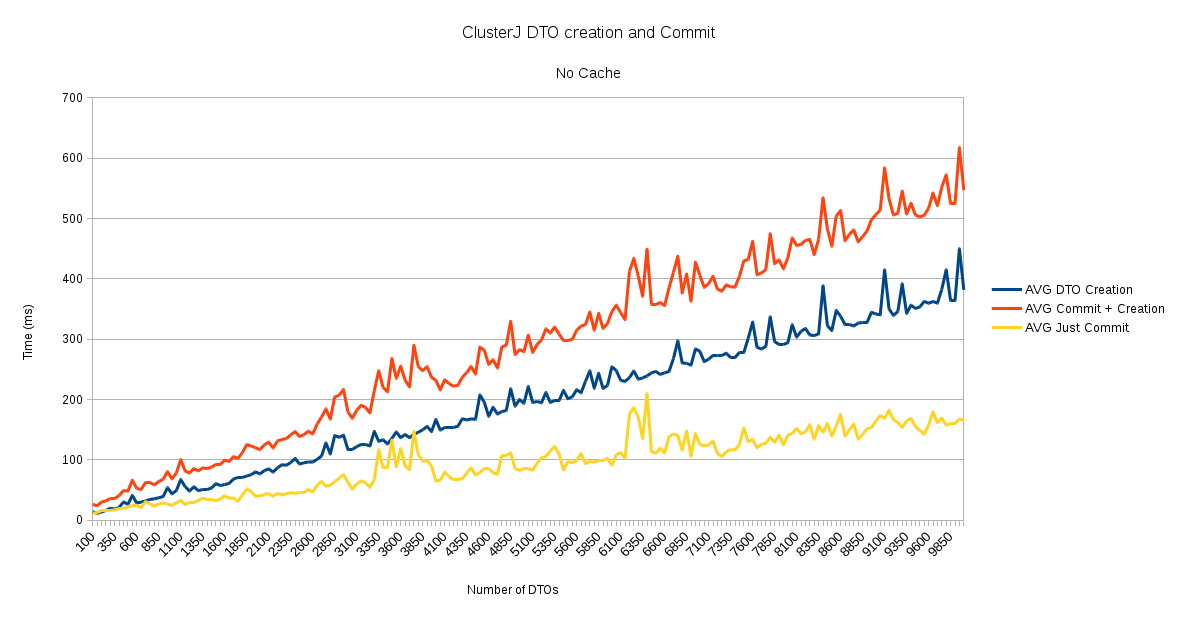
\includegraphics[scale=0.55]{resources/images/Implementation/dto_create_commit_no_cache.png}
\caption{Create and commit time for simple DTOs}
\label{fig:impl_dto_no_cache}
\end{figure}

In ClusterJ, DTOs are created from database \emph{session} object. Creation
of a new DTO involves the instantiation of several objects such as the
handlers for the type of values the DTO will persist in NDB. Upon creation
of all the necessary handlers, it invokes the
\texttt{session.newInstance} reflective method of Java. Java reflection API is
a powerful tool but comes with some pitfalls including
performance \cite{java_reflection}. Reflection API loads types dynamically therefore JVM
optimizations cannot be applied making it a bad candidate for
high-performance applications. Changing the implementation of ClusterJ
is a very difficult task and was not considered as an
option. Moreover, we do not want to maintain one more project.

In Hops, \emph{HopsSession}s are wrapped around ClusterJ sessions. The
solution we designed is a DTO cache for the database sessions.
A session has its own cache space that is filled
up with instances created by the ``slow'' ClusterJ instantiation
process. When we actually need to use a DTO, we fetch it from
the cache which is faster since the objects have already been
created. When the cache has been used a worker thread fills it up
again with new instances. The cache generator service should be used
cautiously. We should not max-out CPUs just for creating cached DTOs, so the
cache is enabled only for a fraction of sessions and only for
heavy-duty DTOs. The reason we decided to have both cache-enabled
and cache-disabled sessions, is to avoid marking a cached session as
used even though the cache was never used. An overall workflow 
of Hops-YARN database session provider
is illustrated in Figure \ref{fig:impl_dto_session_arch}. A
transaction requests a cache-disabled session from the cache-disabled
session pool $(1)$. If there is a session available -- not used by
other transactions -- then the session provider return a session from
the pool, otherwise it creates a new one. When the transaction has
been committed to the database, the session is returned back to the pool
of cache-disabled sessions $(3)$. The workflow for a cache-enabled
session regarding the DB session provider is
different. There are two different cache-enabled session
pools. The first one, \emph{Preparing pool} contains sessions with
their cached used and probably empty. The second pool is the
\emph{Ready pool} with sessions whose cache is full and ready for
usage. When a transaction requests a cache-enabled session, the session
provider first looks on the \emph{Ready pool} $(1)$. If there is an
available session it returns it to the requester $(2)$, otherwise it
looks into the \emph{Preparing pool}. Finally, if there is no session
there either, it creates a new session to NDB. When the transaction
has performed its operations, it returns the session to the
\emph{Preparing pool}. The cache generator service picks sessions from
the \emph{Preparing pool} $(1)$, fills up their cache with the appropriate
DTO instances and places them back to the \emph{Ready pool} $(2)$.

\begin{figure}
\centering
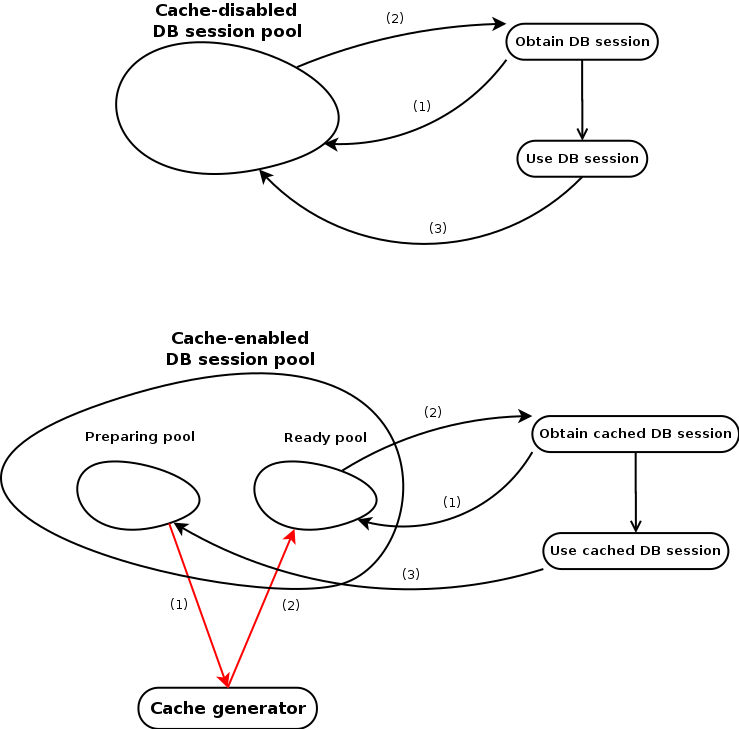
\includegraphics[scale=0.4]{resources/images/Implementation/db_session_pools.png}
\caption{Hops-YARN DB session pool}
\label{fig:impl_dto_session_arch}
\end{figure}

The cache itself, \texttt{DTOCacheImpl} is implemented as a \texttt{ConcurrentHashMap} whose
key is the type of DTO cached and its value is a \texttt{CacheEntry}
object. The \texttt{CacheEntry} is supported by an
\texttt{ArrayBlockingQueue} providing methods for putting and getting
cached objects and increasing the cache size. We will see later how
the size of the cache is increased. For every \texttt{HopsSession}
that has its cache enabled, there is an instance of
\texttt{DTOCacheImpl} which provides methods for (de)registering a DTO
type to the cache and methods that delegate putting and getting objects to the
appropriate \texttt{CacheEntry}. There are
two ways to ``instantiate'' DTO objects. The first one is the
\texttt{newInstance} which makes a call to ClusterJ to create the
object. We use this for non-cached DTO types. The other variation is
the \texttt{newCachedInstance} which makes a call to the cache
instead. In this version the DTO has been instantiated
ahead of time and it is fetched from the cache. The semantics of the
cache is to return the cached object if
it exists in the cache and \texttt{null} if the cache is empty. In
case of an empty cache, we fall back to the ClusterJ instantiation
method. Every \texttt{CacheEntry} keeps track of how many cache-misses
have been occurred. If there are too many, it means that this DTO type
is very demanding and the cache size is increased every time the
cache-misses exceed a certain threshold. So, at the same cache-enabled
session two DTO types might have different cache size depending on
their ``popularity''.

When a cached-enabled session has been used, it is put back in the
\emph{Preparing pool}. The \texttt{DTOCacheGenerator} is a service
that picks sessions from that pool and fills their cache. It removes a
number of sessions from the \emph{Preparing pool} and it spawns threads
that populate every \texttt{CacheEntry} that is not
full. The instantiation of the cached DTO objects is done with the
\texttt{session.newInstance} method of ClusterJ. \texttt{CacheEntry} returns
\texttt{true} for every put, until
the back-end \texttt{ArrayBlockingQueue} is full when it returns
\texttt{false}. When all the \texttt{CacheEntry}s of a session are
full, it (the session) is placed to the \emph{Ready pool} and another
transaction will use it. One note should be made here. ClusterJ
allocates memory for DTO objects out of the heap, with the use of
Java \emph{direct} ByteBuffer. ByteBuffers do not account in Java's
garbage collection mechanism, reducing the GC pause time. Also, they are ideal
for heavy duty I/O operations since JVM does not have to copy data
from intermediate buffers to native buffers. With the caching
mechanism we create more than 6000 DTOs ahead of time per
session and the default direct memory size reaches its limit very
quickly. In order to avoid related exceptions, the flag
\texttt{-XX:MaxDirectMemorySize} should be set to a reasonable value.

\lstinputlisting[float,language=xml,numbers=left,caption={Caching
  mechanism configuration file},label=lst:dto_cache_conf,basicstyle=\footnotesize]{resources/listings/dto-cache-config.xml}

All the parameters for the caching mechanism are specified by a
configuration file, \texttt{dto\_cache-config.xml} in
\texttt{hops-metadata-dal-impl-ndb} that is loaded when
the service starts. A typical example looks like in Listing
\ref{lst:dto_cache_conf}. First, it is specified how many sessions
will have their cache enabled, then a hard limit on the number
of threads that will be created to populate the sessions' cache and
the number of sessions each worker thread will handle. Then in line 14
is the number of sessions in the \emph{Preparing pool} required to
trigger the cache generator threads. If \textbf{sessionsInterval}
$>$ \emph{sessionsPerThread} $*$ \emph{threadLimit}, then some
sessions will be blocked until a thread has finished its work and
scheduled again. Following the mechanism parameters, are the DTO types
that should be cached. In this example we want each cache-enabled
session to cache two types of DTOs. Line 18 is the class name that
encloses the ClusterJ specially decorated interface. Line 21 is the
name of the interface and then follows the initial size of the cache,
the maximum size and the step which the cache size will be increased after some
threshold of cache-misses.

\subsection{Conclusions}
\label{ssec:impl_dto_caching_conslusions}
The caching mechanism explained in this section boosted the
performance of Hops-YARN as it is presented in Chapter \ref{chap:evaluation}. Yet
we have not discovered the advantages in full extend since we need to
experiment more with different types of DTOs. For sure ClusterJ's way
of creating DTOs is not optimal, imposing a great overhead to our system.